% This file was converted to LaTeX by Writer2LaTeX ver. 1.6
% see http://writer2latex.sourceforge.net for more info
\documentclass[a4paper]{article}
\usepackage[utf8]{inputenc}
\usepackage[noenc]{tipa}
\usepackage{tipx}
\usepackage[geometry,weather,misc,clock]{ifsym}
\usepackage{pifont}
\usepackage{eurosym}
\usepackage{amsmath}
\usepackage{wasysym}
\usepackage{amssymb,amsfonts,textcomp}
\usepackage[T3,T1]{fontenc}
\usepackage[varg]{txfonts}\usepackage[polish]{babel}
\usepackage{color}
\usepackage[top=2.499cm,bottom=2.499cm,left=2.499cm,right=2.499cm,nohead,nofoot]{geometry}
\usepackage{array}
\usepackage{hhline}
\usepackage{hyperref}
\hypersetup{pdftex, colorlinks=true, linkcolor=blue, citecolor=blue, filecolor=blue, urlcolor=blue, pdftitle=}
\usepackage[pdftex]{graphicx}
% Footnote rule
\setlength{\skip\footins}{0.119cm}
\renewcommand\footnoterule{\vspace*{-0.018cm}\setlength\leftskip{0pt}\setlength\rightskip{0pt plus 1fil}\noindent\textcolor{black}{\rule{0.25\columnwidth}{0.018cm}}\vspace*{0.101cm}}
\title{}
\begin{document}
{\bfseries
How Many Kingdoms of Life? Eukaryotic Phylogeny and Philosophy of Systematics}

Lukasz Lamza

Copernicus Center for Interdisciplinary Studies, Jagiellonian University in Krakow, Poland

Abstract:

According to contemporary understanding of the universal tree of life, the traditionally recognized kingdoms of
eukaryotic organisms – Protista, Fungi, Animalia and Plantae – are irregularly interspersed in a vast phylogenetic
tree. There are numerous groups that in any Linnaean classification advised by phylogenetic relationships (i.e. a
Hennigian system) would form sister groups to those kingdoms, therefore requiring us to admit them the same rank. In
practice, this would lead to the creation of ca. 25-30 new kingdoms that would now be listed among animals and plants
as “major types of life”. This poses problems of an aesthetic and educational nature. There are, broadly speaking, two
ways to deal with that issue: a) ignore the aesthetic and educational arguments and propose classification systems that
are fully consistent with the Hennigian principles of phylogenetic classification, i.e. are only composed of
monophyletic taxa; b) ignore Hennigian principles and bunch small, relatively uncharacteristic groups into paraphyletic
taxa, creating systems that are more convenient. In the paper, I present the debate and analyze the pros and cons of
both options, briefly commenting on the deeper, third resolution, which would be to abandon classification systems
entirely. Recent advances in eukaryotic classification and phylogeny are commented in the light of the philosophical
question of the purpose and design principles of biological classification systems.

Keywords: Taxonomy; Systematics; Philosophy of Biology; Eukaryotes; Protista

Ever since Linnaeus formalized biological classification in his \textit{Systema Naturae}
\label{ref:RNDRPHrvYOnL2}(Linnaeus, 1788), there is the unresolved problem of how exactly should new taxa be created,
and, more specifically, into how many subtaxa should higher-rank taxa be split. For instance, is there a convincing
reason why there should be, say, 43 orders of ray-finned fish (class Actinopterygii), but only 3 orders of leeches
(class Hirudinea)? Are there any objective arguments for one arrangement over another, or is it purely a matter of
taste? There is a considerable body of work in philosophy of biology that discusses such issues
\label{ref:RNDfhQVj97gMS}(see Hull, 1965, 1970; Schuh and Brower, 2011; and especially Mayr and Bock, 2002).

While ongoing changes at lower ranks (i.e. species, genus, family and order) are of high importance to specialists, the
public is much more likely to encounter changes at the higher ranks (from class up). Of special importance is the
traditionally highest category of kingdom (now partially superseded by domain – see below) which delineates major
“types of life” and is of enormous educational and heuristic value \label{ref:RND3zNGphpm9n}(Copeland, 1938;
Cavalier-Smith, 1981). For centuries there has been slow incremental change in the classification of life at the level
of kingdom. In the recent two decades, however, the rapidly increasing knowledge of the general topology of the
universal tree of life, lead to the realization that traditionally distinguished kingdoms are interspersed in a thick
“bush” of major branches \label{ref:RNDASUVezikg7}(see e.g. Baldauf et al., 2000). In this paper, I wish to analyze
this situation, with special attention to the structure of the eukaryotic tree of life. 

{\bfseries
1. The rank of kingdom}

In biological systematics, starting from Linnaeus, the rank of kingdom has long been the highest of all taxonomic ranks.
In Linnaeus’ \textit{Systema Naturae}, there were 3 of them – the animal, plant and mineral kingdom
\label{ref:RND6bXO1caZ3A}(Linnaeus, 1788), and the division of all living things into two kingdoms was retained in
biology for a long time. Only recently the even higher rank of domain was introduced by Carl Woese
\label{ref:RNDDiuS3oKKqs}(Woese, Kandler and Wheelis, 1990), who intended to accentuate the special character of
Archaea, famously identified by him and George Fox \label{ref:RNDIQY6gpSHPx}(Woese and Fox, 1977) to be fundamentally
different from both bacteria and eukaryotes; although it has been recently suggested that eukaryotes actually evolved
from archaea \label{ref:RND5ULE3HHm08}(Williams et al., 2013). Even in Woese’s 1990 revision, however, three “primary
kingdoms” were named with the idea that the rank of kingdom remains the basic level at which major “types of life” are
to be identified.

The number of the kingdoms of life discerned by biologists changes through time rather slowly. A contemporary student of
both introductory and advanced biological texts is almost certain to encounter the following:

\begin{itemize}
\item either a single kingdom of bacteria, variously called Prokaryotae, Bacteria or Monera, or, in a more modern
variation, two kingdoms: the so-called true bacteria (Eubacteria, sometimes Bacteria) and the archaeans (Archaea,
sometimes Archaebacteria);
\item the single kingdom of protists (usually Protista or Protoctista), which encompasses all eukaryotes not belonging
to the three multicellular kingdoms (see below); in some modern sources \label{ref:RNDdqkS30YvK5}(e.g. Ruggiero et al.,
2015) there is a separate kingdom Chromista encompassing a large monophyletic subgroup of protists, including brown
algae which are large, multicellular and quite complex;
\item the three multicellular eukaryotic kingdoms: plants (Plantae, sometimes Viridiplantae), animals (Animalia,
sometimes Metazoa) and fungi (Fungi, sometimes Mycota). 
\end{itemize}
Note that the list is quite conservative, but the number of kingdoms slowly increases. Plants and  animals are the two
original Linnaean kingdoms of life. Protists were argued to be a separate kingdom by Ernst Haeckel in 1866
\label{ref:RNDnC4UhA8FAD}(Haeckel, 1866). Bacteria were given a separate kingdom in 1938
\label{ref:RNDsDaQPHVHjj}(Copeland, 1938) and, interestingly, the fungi have been proposed as a kingdom separate from
plants only in 1969 \label{ref:RNDzC4ki5UDBu}(Whittaker, 1969). The distinct kingdom for Archaea, as mentioned, was
proposed in 1977 and Thomas Cavalier-Smith first proposed elevating Chromista to the rank of kingdom in 1981
\label{ref:RNDnKGExfa2wY}(Cavalier-Smith, 1981). 

Arguably, the most common variant found in introductory texts is the one with five kingdoms: Bacteria, Protoctista,
Plantae, Animalia, Fungi, and this very division has been employed in the highly influential popular book by Lynn
Margulis and Michael Chapman, \textit{Kingdoms and Domains }\label{ref:RND5xqZMYPEO1}(Margulis and Chapman, 2009),
which has become an authoritative source on biological megasystematics. In a recent proposal of a comprehensive
classification of life, down to the level of order \label{ref:RNDva9PR88ZHQ}(Ruggiero et al., 2015), there are seven
kingdoms: Archaea/Archaebacteria, Bacteria/Eubacteria, Protozoa, Chromista, Fungi, Plantae and Animalia. This proposal
is a consensus view of over 3000 taxonomists (!) and is likely to become the standard point of reference for
professional biologists for years to come, even though it has been criticized, especially with regard to specific
taxonomic decisions \label{ref:RND4kurLEBPnA}(e.g. Tedersoo et al., 2018).

All in all, based on that quick review, it may seem that a general view of the diversity of life, and its representation
in biological taxonomy, is now more or less understood, and major changes to the number of kingdom occur rarely. In
reality, it not that simple. In the past decades there has been considerable controversy surrounding the number and
identity of the highest ranks in systematics, and the summary presented above might be termed the “conservative view”
by some. In fact, there are sources claiming that 11-12 prokaryotic kingdoms \label{ref:RNDXxF0Lm1b0k}(Petitjean et
al., 2014) and 20-27 eukaryotic kingdoms \label{ref:RNDB4YmCpjg7j}(Pawlowski, 2013; Tedersoo, 2017) should be
distinguished.

The purpose of the present paper is to identify the cause of that confusion and its possible resolutions, using mostly
examples related to the eukaryotic tree of life.

{\bfseries
2. Paraphyletic taxa and classification systems}

Starting from Darwin himself, it has become increasingly clear that biological systematics must somehow portray
evolutionary patterns. This was formalized in Willi Hennig’s \textit{Phylogenetic Systematics}
\label{ref:RNDWJhbleZaU4}(Hennig, 1966) where the now-ubiquitous concepts of symplesiomorphy, synapomorphy and
convergence, and the corresponding types of taxa – paraphyletic, monophyletic and polyphyletic – were formalized.
Hennig forcefully argued that valid taxa should only be monophyletic groups, i.e. (true) clades, that is groups of
species composed of \textit{all} descendants of a given species, possessing a common derivative character
(synapomorphy). In the science of cladistics this has since become gospel.

While admirable, this prescription leads to “taxonomical inflation” as more and more taxa are identified. Before we
illustrate it with an example relevant for the present study, let’s consider a case with more familiar taxa.

Vertebrates (subphylum Vertebrata of phylum Chordata) are divided into a number of classes. A popular list of vertebrate
classes that you may hear even from a child (the specific reason for mentioning children in this context will be given
below) is as follows: fish, amphibians, reptiles, birds and mammals. A better-educated person might cite the current
scientific consensus that “fish” should be actually split into a number of separate classes: hagfish (Myxini), lampreys
(Hyperoartia), cartilaginous fish (Chondrichthyes), ray-finned fish (Actinopterygii) and lobe-finned fish
(Sarcopterygii), the reason being that “fish” is actually a paraphyletic grouping. This prescription to discuss five
types of fish, which a layperson may identify as unnecessary and confusing (why five classes of fish and just one class
of birds?), is a first sign of what happens when one attempts to divide a given taxon into monophyletic subtaxa.

If one were to portray the abovementioned vertebrate classes on a phylogenetic tree, something like Fig. 1 might be a
reasonable representation of actual relationships.

{\centering  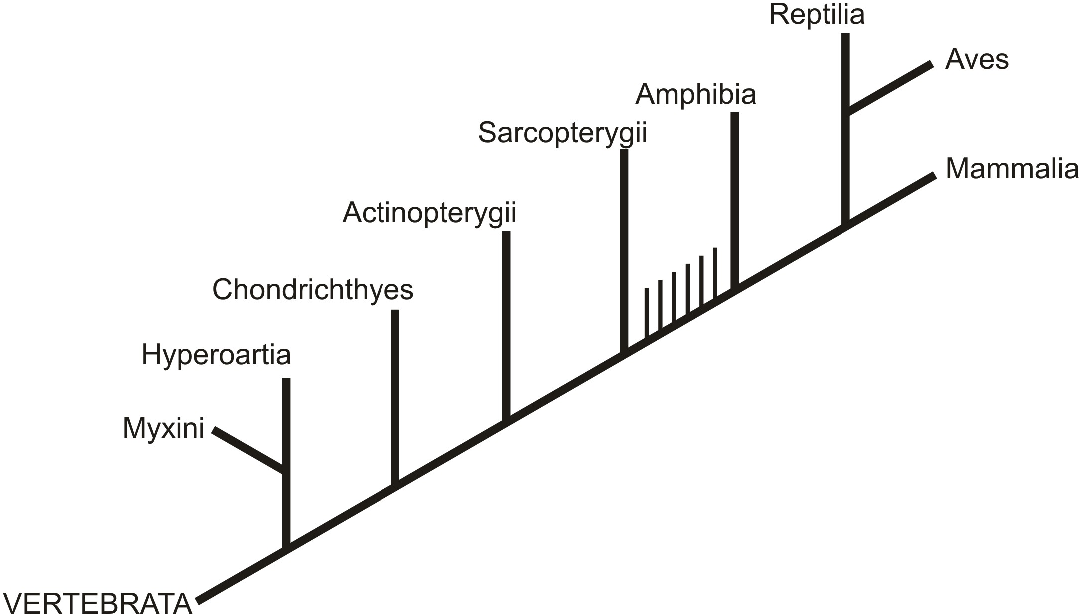
\includegraphics{Lamzaorg-img001.pdf} \par}
\textbf{Fig. 1. }A highly simplified, and ultimately wrong, phylogenetic tree of extant vertebrates that attempts to
include only the extant classes of subphylum Vertebrata. The ‘comb’ represents the area magnified in Fig. 2. It is
clear that one cannot map a ranked classification of extant vertebrate classes onto a valid phylogenetic tree,
especially because of the existence of extinct groups. Specifically, it is impossible to validly represent the actual
relationships between (paraphyletic and now obsolete) Reptilia and Aves (which nest within reptiles).

This is, however, yet another simplification. A more careful analysis of \textit{any }segment of the vertebrate
phylogenetic tree will reveal that in between the well-known groups there are numerous groups, usually extinct, that
would all require classes of their own, if the bordering taxa are given the rank of class – consult Fig. 2.

{\centering  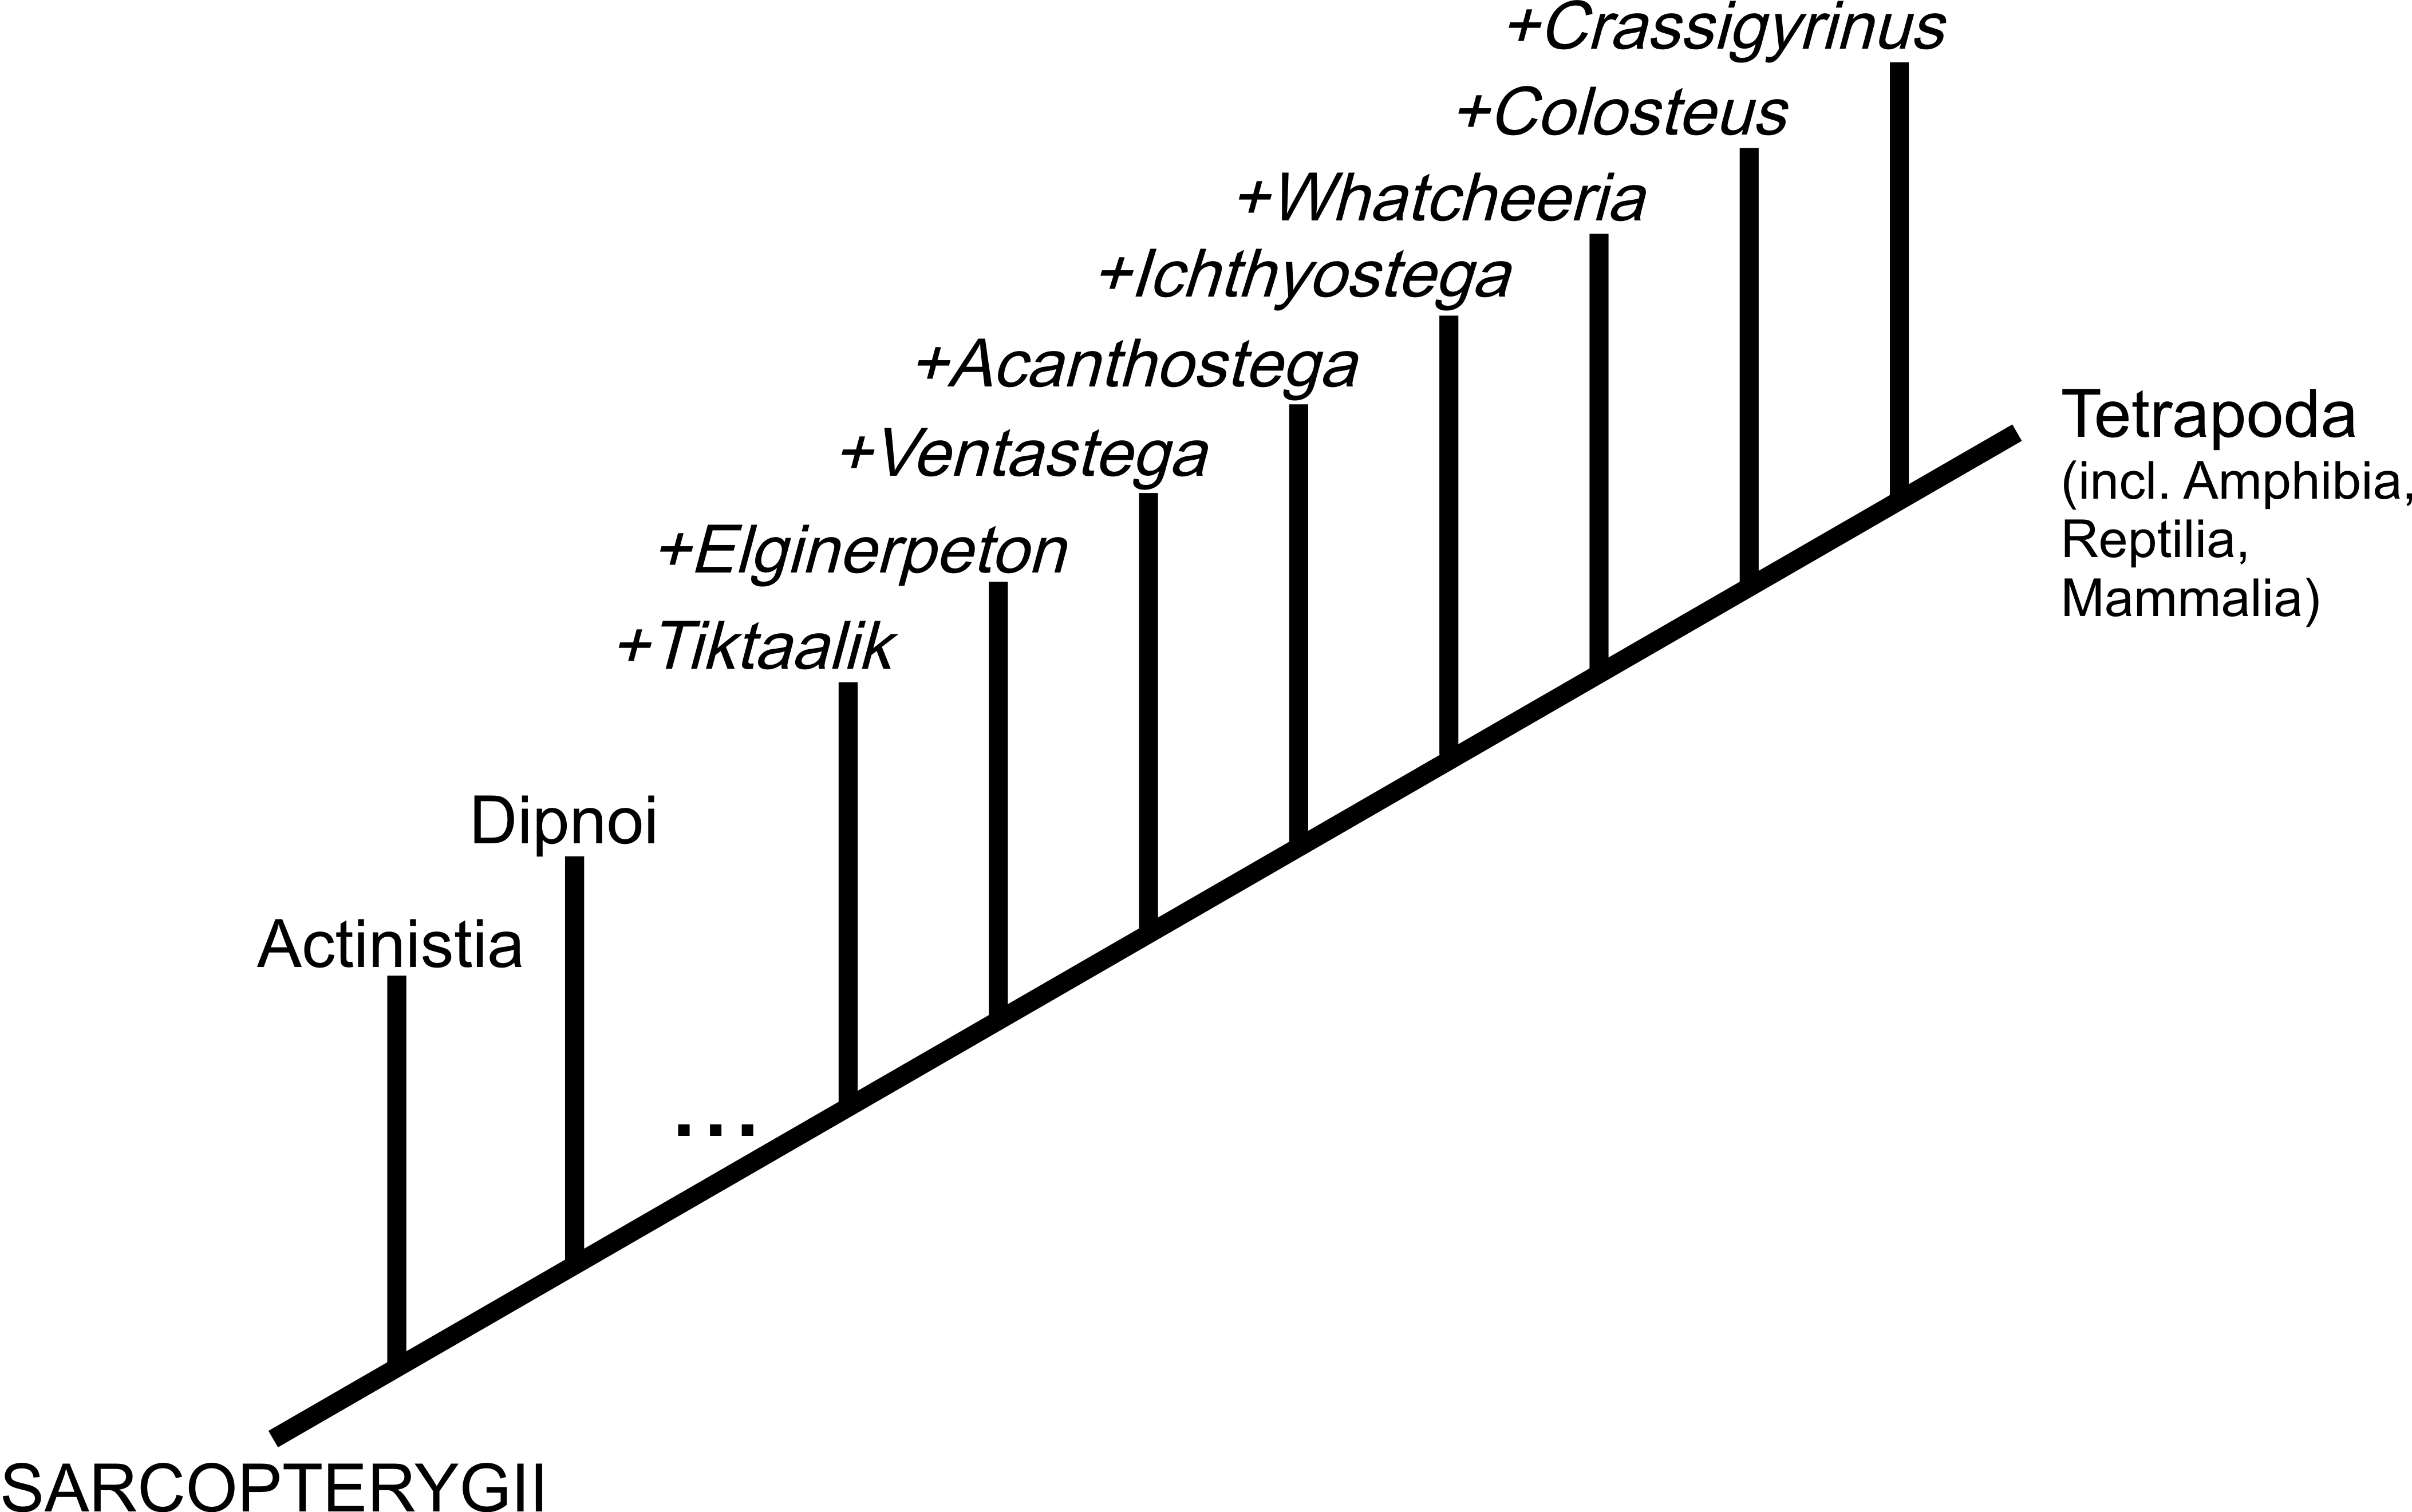
\includegraphics{Lamzaorg-img002.jpg} \par}
\textbf{Fig. 2.} A slightly more realistic representation of a segment of the vertebrate phylogenetic tree, based on
\label{ref:RNDPuknxVrJnD}(Swartz, 2012) (with many taxa removed, most notably a large group of early sarcopterygians,
denoted by an ellipsis). The improvement over Fig. 1 is mostly in that: a) the term Sarcopterygii is now correctly
represented to also include all tetrapods, while in common usage, represented in Fig. 1, it refers only to coelacanths
(which belong to Actinistia) and lungfish (which belong to Dipnoi); b) a number of extinct (marked by a cross) genera
are presented.

It is clear that in order to divide the taxa listed in Fig. 2 into classes, one would have to give each genus presented
in that figure its own high-level taxon (here: most likely class). The alternative is accepting paraphyletic taxa, for
instance by grouping all stem tetrapods (Tiktaalik... Crassigyrinus) in a single class. It clearly goes against
phylogenetic systematics, which is usually defended by biologists working with specific groups of organisms as the only
method of creating taxonomies that is commensurate with the theory of evolution \label{ref:RNDkC4ruFguZT}(see e.g.
Williams and Kociolek, 2007).

There are ways to avoid that, one of which is the so-called sequencing convention proposed by Nelson
\label{ref:RNDHQubFlpSOG}(1972) and developed by Wiley \label{ref:RNDoeFoXTp1sn}(1981) and others, which partly
automates the ranking process in various branches of the phylogenetic tree. But for new, let’s assume that we want to
hold on to strict Hennigian principles; what would be the consequences? Quite simple: the necessity to create a
complete system of monophyletic taxa, in case of vertebrates, would lead to the erection of tens, if not hundreds,
classes of vertebrates which defeats the simplifying purpose of classification. Another solution would be to erect a
large number of taxa of intermediate rank – this has been done, for example, by McKenna \& Bell in their influential
classification of mammals \label{ref:RNDTh5Uw8JZAm}(McKenna and Bell, 1997):

\begin{itemize}
\item class Mammalia

\begin{itemize}
\item subclass Prototheria
\item subclass Theriiformes

\begin{itemize}
\item infraclass +Allotheria
\item infraclass +Eutriconodonta
\item infraclass Holotheria

\begin{itemize}
\item superlegion +Kuehneotheria
\item superlegion Trechnotheria

legion +Symmetrodonta
legion Cladotheria

sublegion +Dryolestoidea
sublegion Zatheria

infralegion +Peramura
infralegion Tribosphenida
...
\end{itemize}
\end{itemize}
\end{itemize}
\end{itemize}
It is worth noting that the authors of that classification are paleontologists and their system is clearly intended as
an answer to the problem of finding a proper taxonomic space for extinct groups. As a result, a staggering number of
ranks were created. In “core Linnaean” taxonomy classes are composed of orders, i.e. class and order are neighboring
ranks. In McKenna \& Bell’s system one will find between them: subclasses, infraclasses, superlegions, legions,
sublegions, infralegions, supercohorts, cohorts, magnorders, superorders, grandorders and mirorders. The term
“taxonomic inflation” may thus have two meanings: the creation of an impractically large number of equally-ranked taxa
and the creation of an impractically large number of ranks.

Let’s now discuss these two alternatives in more detail.

{\bfseries
3. The solutions}

{\bfseries
3.1. Solution I: classifications with only monophyletic taxa}

As mentioned above, strictly adhering to Hennig’s prescription to accept only monophyletic taxa leads to “taxonomic
inflation” – which seems to go against the aesthetic intuition of those biologists who dread the idea of splitting a
given, let’s say, phylum, into 50 classes \label{ref:RNDsx8NDQDrK2}(Cavalier-Smith, 1998).

Surprisingly, the solution that has been commonly employed is to do something perhaps even more drastic: to drop
altogether the Linnaean “logic” of classification which is based on the simple idea that taxa of a given rank are
divided into a number of subordinate taxa of the same lower rank – i.e. kingdoms are divided \textit{only} into phyla;
phyla are divided \textit{only} into classes; classes \textit{only} into orders etc. In other words, every order
belonging to a given phylum must \textit{also }belong to a certain class (or, in some cases, be included as
\textit{incertae sedis}, i.e. temporarily awaiting class attribution). In many modern classifications, however, there
are \textit{missing ranks}. As an example, consider the classification of vertebrates presented by the eminent
paleontologist Michael Benton in his \textit{Vertebrate Palaeontology} \label{ref:RNDqnkTfPlTq8}(Benton, 2014,
p.433nn):

\ding{108} superclass Tetrapoda:

 {\BigCircle} family Elginerpetontidae

 {\BigCircle} \textit{Ventastega}

 {\BigCircle} \textit{Acanthostega}

 {\BigCircle} \textit{Ichthyostega}

 {\BigCircle} \textit{Tulerpeton}

 {\BigCircle} family Colosteidae

 {\BigCircle} family Crassigyrinidae

 {\BigCircle} family Whatcheeriidae

 {\BigCircle} family Baphetidae

 {\BigCircle} class Neotetrapoda [where amphibians, reptiles, birds and mammals can be found – L.L.)

This is a remarkable solution. Note that it clearly opposes the centuries-old tradition, formalized by Linnaeus, to
create consistent, complete hierarchies. Here we have a superclass that is composed of a single class, 5 families and 4
genera.

The missing ranks may look unsettling at first, but this convention is quickly gaining popularity, as it seems to offer
a welcome rescue from the otherwise inescapable alternatives discussed in the previous paragraph. A recent
classification of eukaryotes, published first in 2005 \label{ref:RND5C0kzbt9Jm}(Adl et al., 2005), then in a revised
form in 2012 \label{ref:RND2nC4dhq2C7}(Adl et al., 2012), employs precisely that methodology. Note that this is an
extremely well-respected classification, created by a consortium that includes world-class experts in eukaryotic
diversity (such as Alastair Simpson or Sergei Karpov). The pair of papers is now amongst the most oft-quoted articles
in the field, which means in practice that it is now a point of departure in any discussion of eukaryote
classification.

In both papers the ranks are altogether dropped. Curiously, the taxa are presented in a semi-ordered hierarchical form
where subordinate taxa are given more black dots. For instance, in the earlier paper \label{ref:RNDFR1OTfHJvd}(Adl et
al., 2005) the group Opisthokonta is presented as follows (numerous taxa have been omitted):

OPISTHOKONTA

\ding{108} Fungi

\ding{108}\ding{108} Basidiomycota

\ding{108}\ding{108} Urediniomycetes

\ding{108}\ding{108} Ustilaginomycetes

\ding{108}\ding{108} Ascomycota

\ding{108}\ding{108}\ding{108} \textit{Neolecta}

\ding{108}\ding{108}\ding{108} Taphrinomycotina

...

\ding{108} Mesomycetozoa

\ding{108}\ding{108} Aphelidea

\ding{108}\ding{108} \textit{Corallochytrium}

\ding{108}\ding{108} \textit{Capsaspora}

\ding{108}\ding{108} Ichthyosporea

\ding{108}\ding{108} \textit{Ministeria}

\ding{108}\ding{108} Nucleariida

\ding{108} Choanomonada

\ding{108} Metazoa

\ding{108}\ding{108} Porifera

\ding{108}\ding{108}\ding{108} Silicispongia

\ding{108}\ding{108}\ding{108}\ding{108} Hexactinellida

\ding{108}\ding{108}\ding{108}\ding{108} Demospongiae (...)

Let’s note a few properties of this classification method\textit{.} First of all, the four main groups of Opisthokonta
(the ones with a single dot, i.e. fungi, mesomycetozoans, choanomonads and animals) are, to the best of current
phylogenetic knowledge, monophyletic. This makes them perfect for the role of taxa in an openly Linnaean system, that
is at the same time in line with Hennig’s rules of phylogenetic classification. The taxa with the same number of dots,
however, represent radically different ranks in previously published classifications. The group Mesomycetozoa, as
presented here, is composed of three genera (\textit{Corallochytrium}, \textit{Capsaspora} and \textit{Ministeria}),
two classes (Aphelidea and Ichthyosporea) and one order (Nucleariida). One might of course erect classes for all of
them, which however, often leads to taxonomic inflation, as mentioned in the previous section.

Let’s now specifically discuss the problem of kingdoms. If we hold on to the idea that equal “ranks” in the
classification by Adl \textit{et al.} should be given equal Linnaean ranks, we would be forced to create two additional
kingdoms Choanomonada and Mesomycetozoa, that would be placed alongside Fungi and Metazoa/Animalia in the, most likely,
superkingdom Opisthokonta (plus other kingdoms in other superkingdoms). That is, in fact, a fairly popular point of
view, expressed for instance by Tedersoo \label{ref:RNDXAoIqIPayD}(2017), who includes kingdoms Choanoflagellozoa
(essentially synonymous with Adl \textit{et al.}’s Choanomonada) and Ichthyosporia (Ichthyosporea is a synonym of
Mesomycetozoa in many classification systems). It is worth noting that Tedersoo’s system might be thought of as a good
demonstration of what happens if one attempts to create a Linnaean system adhering to Hennigian constraints, based on
modern understanding of eukaryotic phylogeny (the classification by Adl \textit{et al.} is listed by Tedersoo as one of
his main sources of information). The result? His system has 32 eukaryotic kingdoms. Let’s cite his own opinion on that
fact: “In the proposed classification, the erection of 32 eukaryote kingdoms certainly catches and, perhaps, scratches
the eye. I found adoption of multiple kingdoms necessary to follow the monophyly principle […].”
\label{ref:RNDP7J0D4JTk6}(Tedersoo, 2017, p.8)

Note that Adl \textit{et al. }themselves stand \textit{against }such practices, calling such artificially created
higher-level taxa “superfluous”  \label{ref:RNDTkKC0gomXM}(Adl et al., 2012, p.430), therefore openly arguing for
classification with missing taxa.

{\bfseries
3.2. Solution II: classifications with paraphyletic taxa}

The most vocal contemporary proponent of that solution is probably Thomas Cavalier-Smith, a controversial figure among
microbiologists, who, however, is at the same time undoubtedly one of the most influential personas in the field of
eukaryotic systematics. His contributions include the early recognition, and naming, of Excavata, Opisthokonta,
Rhizaria and Chromista – all of them being now largely accepted, and the latter three: most likely monophyletic,
mega-grouping of eukaryotes. In his proposed classification of life (with six kingdoms)
\label{ref:RNDScaXMIFqT5}(Cavalier-Smith, 1998) there is a long section on “philosophical preliminaries”, where the
necessity for admitting paraphyletic taxa is forcefully defended. His two main arguments against the Hennigian
requirement to limit taxa to clades are as follows:

1) It leads to instability. Each new discovery in biology – be it a paleontological or molecular novelty, or simply the
discovery of a new species or a reinterpretation of anatomical data – may lead to the reassessment of a monophyletic
taxon as paraphyletic, which would force the biologists to update classification systems. In practice it would mean
hundreds, if not thousands, of revisions every year.

2) It is not practical. Let’s quote Cavalier-Smith himself: “Whether a taxon is paraphyletic or not is irrelevant to its
validity as a taxon. It is also irrelevant to many of the uses to which classifications are put, such as arranging
specimens in a museum, organising the chapters in a biology textbook, or providing a convenient label, e.g. bacteria or
fungi, for a group of similar organisms.” \label{ref:RNDUlTuwI9YEO}(Cavalier-Smith, 1998, p.212)

As a result, Cavalier-Smith for about two decades has become an active opponent of Hennigian classification, especially
in the field of microbiology. Every year or two he proposes a new system of classification, sometimes general, most
often specific to a group of eukaryotes \label{ref:RNDtoAIslWhri}(see e.g. Cavalier-Smith, 2002, 2013, 2016), usually
being a carefully crafted compromise between contemporary phylogenetic knowledge and practicality. His 1998 system
\label{ref:RNDJbJ6dU4tG1}(Cavalier-Smith, 1998) has six kingdoms:

\begin{itemize}
\item empire/superkingdom Prokaryota*

\begin{itemize}
\item kingdom Bacteria* [note: Archaebacteria are to be found here, as an infrakingdom]
\end{itemize}
\item empire/superkingdom Eukaryota

\begin{itemize}
\item kingdom Protozoa*

\begin{itemize}
\item subkingdom Archezoa*
\item subkingdom Neozoa*
\end{itemize}
\item kingdom Animalia
\item kingdom Fungi
\item kingdom Plantae
\item kingdom Chromista
\end{itemize}
\end{itemize}
All openly paraphyletic (“almost certainly paraphyletic” in his own words) taxa are marked with an asterisk. It is
interesting to note that, while Cavalier-Smith openly opposes Hennigian phylogenetic systematics, his “illegal”
taxonomies are highly popular. A quick look into any contemporary paper on eukaryotic systematics will reveal a number
of high-level taxa formally defined by Cavalier-Smith, many of them known or suspected to be paraphyletic. The reason
is simple: his classifications are extremely convenient, because they are invariably composed in such a way as to
include only a minimal number of taxa \textit{and} ranks which are \textit{usually }monophyletic, but sometimes are
paraphyletic if that makes for a convenient system. The reader is referred to the above-cited paper (Cavalier-Smith,
1998) where his philosophy of biological classification is explained in detail.

On a side, and probably more personal, note: the zoologists reading this paper may find it interesting to go through his
proposed classification of the animal kingdom \label{ref:RNDayLTgHPurs}(Cavalier-Smith, 1998, pp.235–237) which offers,
in the opinion of the author of this paper, a refreshing look at the list of animal phyla. As currently recognized,
there is somewhere around 30-35 phyla – consult any modern textbook on zoology – that only recently began to be grouped
into a few large monophyletic groups, such as Spiralia, Ecdysozoa or Deuterostomia. Other than that, there is a
confusing diversity of tiny phyla, most of them unknown to the general public: how many non-zoologists know of
Kinorhyncha, Loricifera, Gnathostomulida (jaw worms) or Acanthocephala (spiny-headed worms)? Cavalier-Smith groups all
animals into 22 phyla – still a long list, but, especially with the aid of his clear, succinct diagnoses, is much more
manageable. The classification includes some, but rather few, paraphyletic taxa.

{\bfseries
3.3. Solution III: abandon classification systems}

The third solution would be to run away from the problem, so to speak, and refrain from explicitly writing down
classifications, and discuss biological diversity through phylogenetic trees only. This has been proposed from time to
time by certain scientists and philosophers (the proposal has been reviewed and critiqued by Michael Benton
\label{ref:RNDvl4WtKWtke}(2000)). While reading biological literature, one finds this sentiment expressed from time to
time, especially by specialists working with rapidly changing classification systems. There is a fascinating, heated
dialogue that ensued during the 1970 First International Conference on Ephemeroptera, recorded in this conference’s
proceedings \label{ref:RNDKBHKSFREeT}(Peters and Peters, 1973, pp.151–154), where a group of entomologists become
increasingly frustrated by their inability to create a classification system based on the otherwise clear phylogenetic
evidence presented by one of the participants \label{ref:RNDRwD3oy2Fl1}(Edmunds Jr, 1973). In fact, all the problems
discussed in this paper with regard to higher ranks are mentioned during that discussion, which is about families,
subfamilies and genera of Ephemeroptera, which makes for a great read.

There are at least two large groups in biology that have abandoned updating the classification of the organisms they are
working with: botanists working with flowering plants and malacologists.

In the first case, one would be hard-pressed to find a recent authoritative classification of flowering plants, because
the focus of the communal effort has long been the creation of better and better phylogenies, not taxonomies. The
Angiosperm Phylogeny Group regularly publishes the new view on plant phylogeny, employing formal taxa only to the level
of order \label{ref:RNDly7gwmyvG1}(see e.g. Chase et al., 2016). All the higher-rank taxa are abandoned, and no
higher-rank taxonomies are officially accepted by APG.

The exactly same process had happened in the field of malacology, where for years there were no formal definitions of
gastropod taxa above the level of superfamily \label{ref:RND5saL769IKK}(see Bouchet and Rocroi, 2005). Interestingly,
the situation visibly upset some of the workers in the field who started spontaneously grouping the newly defined
families and superfamilies into orders, those into superorders, subclasses etc. Last year in a revision of the 2005
classification \label{ref:RNDSnxh8fRQNP}(Bouchet et al., 2017), the authors surrendered and included higher-ranked
taxa, although the system is now very “messy”: it includes numerous intermediate-level ranks that correspond to the
unranked clades in the previous classification – there are classes, subclasses, infraclasses, cohorts, subcohorts,
superorders, orders, suborders and infraorders in the system, plus a handful of openly paraphyletic “grades”. The
struggle of malacologists to bring back Linnaean classification into the world of Hennigian unranked lists à la Adl
\textit{et al.} leads to exactly the same problems that were discussed in the previous sections.

The case of gastropod classification illustrates, however, that even specialists working in very narrow fields need
balanced ranked classification systems. It is not only for the purposes of educating the young, writing books or
organizing museum expositions that we need neat, logical classifications with no missing ranks and a small number of
distinctive, easy to remember taxa. The specialists need them too. The option to abandon classification systems seems
to be not viable, especially that it is both trivial and tempting to create a list of clades from a phylogenetic tree,
adding ranks to some or all taxa, which would be a \textit{de facto} classification, just like Benton did in his
\textit{Vertebrate Palaeontology}.

{\bfseries
4. Summary}

Our increasing knowledge of biodiversity, especially in the case of microbiology, both prokaryotic and eukaryotic, will
inevitably lead to the escalation of the problems presented in this paper. Because it doesn’t seem plausible that
classification systems will be altogether abandoned (which would leave us only with phylogenetic trees, sometimes
presented as unranked lists), it seems that we must somehow solve the problem of creating classification systems in the
times of abundant phylogenetic data.

Broadly speaking, there seem to be two directions that one might take: 1) to follow phylogenetic data to the letter; 2)
to follow intuition and convenience. Simply put, the option 1) would mean having only proper monophyletic taxa, but a
highly impractical system; and the option 2) would mean having also paraphyletic taxa \textit{and} a system that is
practical.

In the special case of eukaryotic kingdoms, the first route would lead to a revolution in biological classification of
life and numerous kingdoms currently unknown to the general public would be introduced
\label{ref:RND3uML7k6B2X}(Tedersoo, 2017), such as Oxymonada, Breviatea or Filasteriae, that would now be listed
alongside plants, animals and fungi as “major types of life”. Alternatively, one might drop the traditional kingdoms
altogether and define the currently recognized eukaryotic “supergroups” \label{ref:RNDsc7VI9vP7w}(e.g. Keeling et al.,
2005) as kingdoms, and what we know recognize as kingdoms would have to be downranked into subkingdoms or
“microkingdoms” \label{ref:RNDAlF3xlGnxL}(Pawlowski, 2013). This would be the resulting classification:

\begin{itemize}
\item kingdom Excavata
\item kingdom Amoebozoa
\item kingdom Opisthokonta (incl. fungi and animals)
\item kingdom Archaeplastida (incl. plants)
\item kingdom Rhizaria
\item kingdom Alveolata
\item kingdom Heterokonta
\end{itemize}
Obviously, this would \textit{not} solve the problem, if one would stubbornly keep on sticking to Hennigian rules. First
of all, Excavata may be paraphyletic \label{ref:RNDd85mwMFAal}(He et al., 2014), in which case we would have to split
it into monophyletic groups, resulting in a classification system alike to this:

\begin{itemize}
\item kingdom Euglenozoa (former Excavata)
\item kingdom Heterolobosea (former Excavata)
\item kingdom Jakobea (former Excavata)
\item kingdom Metamonada (former Excavata)
\item kingdom Amoebozoa
\item kingdom Opisthokonta (incl. fungi and animals)
\item kingdom Archaeplastida (incl. plants)
\item kingdom Rhizaria
\item kingdom Alveolata
\item kingdom Heterokonta
\end{itemize}
Secondly, there is at least a dozen groups of eukaryotes that don’t fit neatly into any of the supergroups, including
\textit{Tsukubamonas} and \textit{Malawimonas}, Cavalier-Smith’s Varisulca, Apusozoa, but also much better-known groups
such as Cryptophyta or Haptophyta. Consequently, in Tedersoo’s system, there \textit{are} kingdoms Malawimonada,
Tsukubamonada, Apusozoa, Cryptista and Haptista which brings us to square one. Obviously, replacing traditional
kingdoms with eukaryotic supergroups is \textit{not }a solution.

The second option – to retain the general structure of the present classification of life into kingdoms – is not fully
satisfactory, either, because the old kingdom Protozoa is now known to be a large, highly structured group that
deserves proper recognition and can’t be rightfully treated as an unstructured bunch of “amoeba and such”
\label{ref:RNDBkv0g8EycM}(see Patterson, 1999). Its representatives have very little in common with each other and
include multicellular forms similar to fungi (mycetozoan slime molds, acrasids) and plants (brown algae), single-celled
large predatory heterotrophs (ciliates), intracellular parasites (kinetoplastids) and endosymbionts (syndineas);
colonial filtrators (choanoflagellates), multinucleate “superamoebae” (labyrinthulomycetes) and tens of other forms.
Small steps, such as Cavalier-Smith’s proposal for the kingdom of Chromista, might be seen a sign of a more
conservative process of a slow, incremental change, not dictated by blind adherence to formalized ideals, but rather by
educational values.

At the moment it is uncertain which approach will dominate, but it’s clear that creating a top-level classification of
life congruent with our contemporary knowledge of eukaryote phylogeny will require us to resign from at least some
philosophical principles of biological systematics.

{\bfseries
References}

\begin{enumerate}
\item Adl, S.M., Simpson, A.G.B., Farmer, M.A., Andersen, R.A., Anderson, O.R., Barta, J.R., Bowser, S.S., Brugerolle,
G., Fensome, R.A., Fredericq, S., James, T.Y., Karpov, S., Kugrens, P., Krug, J., Lane, C.E., Lewis, L.A., Lodge, J.,
Lynn, D.H., Mann, D.G., McCourt, R.M., Mendoza, L., Moestrup, O., Mozley-Standridge, S.E., Nerad, T.A., Shearer, C.A.,
Smirnov, A.V., Spiegel, F.W. and Taylor, M.F.J.R., 2005. The new higher level classification of eukaryotes with
emphasis on the taxonomy of protists. \textit{The Journal of Eukaryotic Microbiology}, 52(5), pp.399–451.
\item Adl, S.M., Simpson, A.G.B., Lane, C.E., Lukeš, J., Bass, D., Bowser, S.S., Brown, M.W., Burki, F., Dunthorn, M.,
Hampl, V., Heiss, A., Hoppenrath, M., Lara, E., Le Gall, L., Lynn, D.H., McManus, H., Mitchell, E.A.D.,
Mozley-Stanridge, S.E., Parfrey, L.W., Pawlowski, J., Rueckert, S., Shadwick, L., Shadwick, L., Schoch, C.L., Smirnov,
A. and Spiegel, F.W., 2012. The revised classification of eukaryotes. \textit{The Journal of Eukaryotic Microbiology},
59(5), pp.429–493.
\item Baldauf, S.L., Roger, A.J., Wenk-Siefert, I. and Doolittle, W.F., 2000. A kingdom-level phylogeny of eukaryotes
based on combined protein data. \textit{Science}, [online] 290(5493), pp.972–977. Available at:
{\textless}https://science.sciencemag.org/content/290/5493/972{\textgreater}.
\item Benton, M.J., 2000. Stems, nodes, crown clades, and rank-free lists: is Linnaeus dead? \textit{Biological
Reviews}, [online] 75(4), pp.633–648. Available at:
{\textless}https://onlinelibrary.wiley.com/doi/abs/10.1111/j.1469-185X.2000.tb00055.x{\textgreater} [Accessed 28 May
2019].
\item Benton, M.J., 2014. \textit{Vertebrate Palaeontology}. Fourth edition ed. Chichester, West Sussex; Hoboken, NJ:
Wiley Blackwell.
\item Bouchet, P. and Rocroi, J.-P., 2005. Classification and nomenclator of gastropod families. \textit{Malacologia:
International Journal of Malacology}, 47(1–2), pp.1–397.
\item Bouchet, P., Rocroi, J.-P., Hausdorf, B., Kaim, A., Kano, Y., Nützel, A., Parkhaev, P., Schrödl, M. and Strong,
E.E., 2017. Revised Classification, Nomenclator and Typification of Gastropod and Monoplacophoran Families.
\textit{Malacologia}, [online] 61(1–2), pp.1–526. Available at:
{\textless}https://bioone.org/journals/Malacologia/volume-61/issue-1-2/040.061.0201/Revised-Classification-Nomenclator-and-Typification-of-Gastropod-and-Monoplacophoran-Families/10.4002/040.061.0201.full{\textgreater}
[Accessed 28 May 2019].
\item Cavalier-Smith, T., 1981. Eukaryote kingdoms: Seven or nine? \textit{Biosystems}, [online] 14(3), pp.461–481.
Available at: {\textless}http://www.sciencedirect.com/science/article/pii/0303264781900502{\textgreater} [Accessed 28
May 2019].
\item Cavalier-Smith, T., 1998. A revised six-kingdom system of life. \textit{Biological Reviews}, [online] 73(3),
pp.203–266. Available at:
{\textless}https://onlinelibrary.wiley.com/doi/abs/10.1111/j.1469-185X.1998.tb00030.x{\textgreater}.
\item Cavalier-Smith, T., 2002. The phagotrophic origin of eukaryotes and phylogenetic classification of Protozoa.
\textit{International Journal of Systematic and Evolutionary Microbiology}, 52(2), pp.297–354.
\item Cavalier-Smith, T., 2013. Early evolution of eukaryote feeding modes, cell structural diversity, and
classification of the protozoan phyla Loukozoa, Sulcozoa, and Choanozoa. \textit{European Journal of Protistology},
49(2), pp.115–178.
\item Cavalier-Smith, T., 2016. Higher classification and phylogeny of Euglenozoa. \textit{European Journal of
Protistology}, [online] 56, pp.250–276. Available at:
{\textless}http://www.sciencedirect.com/science/article/pii/S0932473916300839{\textgreater} [Accessed 28 May 2019].
\item Chase, M.W., Christenhusz, M.J.M., Fay, M.F., Byng, J.W., Judd, W.S., Soltis, D.E., Mabberley, D.J., Sennikov,
A.N., Soltis, P.S. and Stevens, P.F., 2016. An update of the Angiosperm Phylogeny Group classification for the orders
and families of flowering plants: APG IV. \textit{Botanical Journal of the Linnean Society}, [online] 181(1), pp.1–20.
Available at: {\textless}https://academic.oup.com/botlinnean/article/181/1/1/2416499{\textgreater} [Accessed 28 May
2019].
\item Copeland, H.F., 1938. The Kingdoms of Organisms. \textit{The Quarterly Review of Biology}, [online] 13(4),
pp.383–420. Available at: {\textless}https://www.jstor.org/stable/2808554{\textgreater} [Accessed 28 May 2019].
\item Edmunds Jr, G.F., 1973. Some critical problems of family relationships in the Ephemeroptera. In: W.L. Peters and
J.G. Peters, eds., \textit{Proceedings of the First International Conference on Ephemeroptera. Florida Agriculture and
Mechanical University, August 17-20, 1970}. [online] Leiden: Brill, pp.145–154. Available at:
{\textless}https://brill.com/view/title/4058{\textgreater} [Accessed 28 May 2019].
\item Haeckel, E., 1866. \textit{Generelle morphologie der organismen. Allgemeine grundzüge der organischen
formen-wissenschaft, mechanisch begründet durch die von Charles Darwin reformirte descendenztheorie.  2. bd. Allgemeine
entwickelungsgeschichte der organismen}. [online] Berlin: Verlag von G. Reimer. Available at:
{\textless}https://www.biodiversitylibrary.org/bibliography/3953{\textgreater}.
\item He, D., Fiz-Palacios, O., Fu, C.-J., Fehling, J., Tsai, C.-C. and Baldauf, S.L., 2014. An alternative root for the
eukaryote tree of life. \textit{Current Biology}, [online] 24(4), pp.465–470. Available at:
{\textless}https://www.cell.com/current-biology/abstract/S0960-9822(14)00069-4{\textgreater} [Accessed 28 May 2019].
\item Hennig, W., 1966. \textit{Phylogenetic Systematics}. Translated by D. Davis. and Translated by R. Zangerl.
Chicago, Ill.: University of Illinois Press.
\item Hull, D.L., 1965. The effect of essentialism on taxonomy—two thousand years of stasis (I). \textit{The British
Journal for the Philosophy of Science}, [online] 15(60), pp.314–326. Available at:
{\textless}https://academic.oup.com/bjps/article/XV/60/314/1516311{\textgreater} [Accessed 28 May 2019].
\item Hull, D.L., 1970. Contemporary Systematic Philosophies. \textit{Annual Review of Ecology and Systematics},
[online] 1(1), pp.19–54. Available at:
{\textless}https://www.annualreviews.org/doi/10.1146/annurev.es.01.110170.000315{\textgreater} [Accessed 28 May 2019].
\item Keeling, P.J., Burger, G., Durnford, D.G., Lang, B.F., Lee, R.W., Pearlman, R.E., Roger, A.J. and Gray, M.W.,
2005. The tree of eukaryotes. \textit{Trends in Ecology \& Evolution}, [online] 20(12), pp.670–676. Available at:
{\textless}https://www.cell.com/trends/ecology-evolution/abstract/S0169-5347(05)00304-6{\textgreater} [Accessed 28 May
2019].
\item Linnaeus, C., 1788. \textit{Systema naturae per regna tria naturae: secundum classes, ordines, genera, species,
cum characteribus, differentiis, synonymis, locis (vol. 9)}. [online] Lipsiae [Leipzig]: Impensis Georg Emanuel Beer,.
Available at: {\textless}https://www.biodiversitylibrary.org/bibliography/545{\textgreater}.
\item Margulis, L. and Chapman, M.J., 2009. \textit{Kingdoms and Domains: An Illustrated Guide to the Phyla of Life on
Earth}. 4th ed. ed. London: Academic Press.
\item Mayr, E. and Bock, W.J., 2002. Classifications and other ordering systems. \textit{Journal of Zoological
Systematics and Evolutionary Research}, [online] 40(4), pp.169–194. Available at:
{\textless}https://onlinelibrary.wiley.com/doi/abs/10.1046/j.1439-0469.2002.00211.x{\textgreater} [Accessed 28 May
2019].
\item McKenna, M.C. and Bell, S.K., 1997. \textit{Classification of Mammals: Above the Species Level}. New York:
Columbia University Press.
\item Nelson, G.J., 1972. Phylogenetic relationship and classification. \textit{Systematic Biology}, [online] 21(2),
pp.227–231. Available at: {\textless}https://academic.oup.com/sysbio/article/21/2/227/1713485{\textgreater} [Accessed
28 May 2019].
\item Patterson, D.J., 1999. The Diversity of Eukaryotes. \textit{The American Naturalist}, 154(S4), pp.S96–S124.
\item Pawlowski, J., 2013. The new micro-kingdoms of eukaryotes. \textit{BMC Biology}, [online] 11(1), p.40. Available
at: {\textless}http://www.biomedcentral.com/1741-7007/11/40{\textgreater} [Accessed 28 May 2019].
\item Peters, W.L. and Peters, J.G. eds., 1973. \textit{Proceedings of the First International Conference on
Ephemeroptera. Florida Agriculture and Mechanical University, August 17-20, 1970}. [online] Leiden: Brill. Available
at: {\textless}https://brill.com/view/title/4058{\textgreater} [Accessed 28 May 2019].
\item Petitjean, C., Deschamps, P., López-García, P. and Moreira, D., 2014. Rooting the domain Archaea by phylogenomic
analysis supports the foundation of the new kingdom Proteoarchaeota. \textit{Genome Biology and Evolution}, [online]
7(1), pp.191–204. Available at: {\textless}https://www.ncbi.nlm.nih.gov/pmc/articles/PMC4316627/{\textgreater}
[Accessed 28 May 2019].
\item Ruggiero, M.A., Gordon, D.P., Orrell, T.M., Bailly, N., Bourgoin, T., Brusca, R.C., Cavalier-Smith, T., Guiry,
M.D. and Kirk, P.M., 2015. A Higher Level Classification of All Living Organisms. \textit{PLOS ONE}, [online] 10(4),
p.e0119248. Available at:
{\textless}https://journals.plos.org/plosone/article?id=10.1371/journal.pone.0119248{\textgreater} [Accessed 28 May
2019].
\item Schuh, R.T. and Brower, A.V.Z., 2011. \textit{Biological Systematics: Principles and Applications}. [online]
Ithaca, NY: Cornell University Press. Available at: {\textless}https://doi.org/10.7591/9780801462436{\textgreater}
[Accessed 28 May 2019].
\item Swartz, B., 2012. A marine stem-tetrapod from the Devonian of western North America. \textit{PLOS ONE}, [online]
7(3), p.e33683. Available at:
{\textless}https://journals.plos.org/plosone/article?id=10.1371/journal.pone.0033683{\textgreater} [Accessed 28 May
2019].
\item Tedersoo, L., 2017. Proposal for practical multi-kingdom classification of eukaryotes based on monophyly and
comparable divergence time criteria. \textit{bioRxiv}, [online] p.240929. Available at:
{\textless}https://www.biorxiv.org/content/10.1101/240929v1{\textgreater} [Accessed 28 May 2019].
\item Tedersoo, L., Sánchez-Ramírez, S., Kõljalg, U., Bahram, M., Döring, M., Schigel, D., May, T., Ryberg, M. and
Abarenkov, K., 2018. High-level classification of the Fungi and a tool for evolutionary ecological analyses.
\textit{Fungal Diversity}, [online] 90(1), pp.135–159. Available at:
{\textless}https://doi.org/10.1007/s13225-018-0401-0{\textgreater} [Accessed 28 May 2019].
\item Whittaker, R.H., 1969. New concepts of kingdoms of organisms. \textit{Science}, [online] 163(3863), pp.150–160.
Available at: {\textless}https://science.sciencemag.org/content/163/3863/150{\textgreater} [Accessed 28 May 2019].
\item Wiley, E.O., 1981. \textit{Phylogenetics: The Theory and Practice of Phylogenetic Systematics}. New York: John
Wiley.
\item Williams, D.M. and Kociolek, J.P., 2007. Pursuit of a natural classification of diatoms: History, monophyly and
the rejection of paraphyletic taxa. \textit{European Journal of Phycology}, [online] 42(3), pp.313–319. Available at:
{\textless}https://doi.org/10.1080/09670260701419921{\textgreater} [Accessed 28 May 2019].
\item Williams, T.A., Foster, P.G., Cox, C.J. and Embley, T.M., 2013. An archaeal origin of eukaryotes supports only two
primary domains of life. \textit{Nature}, [online] 504(7479), pp.231–236. Available at:
{\textless}https://www.nature.com/articles/nature12779{\textgreater} [Accessed 28 May 2019].
\item Woese, C.R. and Fox, G.E., 1977. Phylogenetic structure of the prokaryotic domain: The primary kingdoms.
\textit{Proceedings of the National Academy of Sciences}, [online] 74(11), pp.5088–5090. Available at:
{\textless}https://www.pnas.org/content/74/11/5088{\textgreater} [Accessed 28 May 2019].
\item Woese, C.R., Kandler, O. and Wheelis, M.L., 1990. Towards a natural system of organisms: proposal for the domains
Archaea, Bacteria, and Eucarya. \textit{Proceedings of the National Academy of Sciences}, [online] 87(12),
pp.4576–4579. Available at: {\textless}https://www.pnas.org/content/87/12/4576{\textgreater} [Accessed 28 May 2019].
\end{enumerate}
\end{document}
